\subsection{Two effects of narrow resonance}
There are two possibilities for narrow resonance:  
\begin{enumerate}
\item Pauli exclusion for three species, where the close-channel weight is large.  
\item Fermi energy is larger than the width that scattering amplitude (NOT $a_{s}$) changes the sign.  Therefore $a_{s}$ is no longer a good indicator for the interaction.  However, it might still be OK to take $a_{s}$ simply as the quantity introduced by renormalization.   This has been explored by several papers already \cite{NarrowJensen1,NarrowJensen,GurarieNarrow}.  
\end{enumerate}
Four species case can fall into narrow resonance in  the second sense.  \cite{NarrowJensen1,NarrowJensen} uses the single-channel approach but a T-matrix with effective range $r_{0}$, the narrow resonance is $r_{0}k_{F}\ll1$.  In \cite{NarrowJensen}, a single-channel bare interaction is assumed and (unnormalized) gap, number equations  are  solved numerically with different interaction parameters corresponding to different effective ranges. The result is some small corrections in gap, chemical potential...   It is not a two-channel treatment.  

\cite{GurarieNarrow} treats the problem in two-channel (molecule+fermi).  The criteria for narrowness is similar.  There are couple of points not clear to me.   
\begin{itemize}
\item Two channels are treated separately, more in He3-A fashion.  The ansatz I used is more in He3-B fashion where two channels are mixed at the very beginning.   According to \cite{He3B}, in He3 He3-B wave-function has lower energy.  What is the case here?

The very procedure to integrate the Fermionic degree of freedom first and look for stable point for bosonic degree of freedom.  How does that affect anything? 

\item The hamilton has no direct interaction in open-channel, which contributes little in resonance.  But it does play some role.  How does that work for my model? 

This smear the open-channel momentum distribution, and further introduce the close-channel component from the coupling before close-channel bound state is energetic favorable.  

\item The claim that the small factor $\gamma=1/(r_{0}k_{F})$ is a little worrisome as a BCS state is non-analytic for any small factor, therefore, the expansion might not cover the BCS-type state, which we are seeking.  
\end{itemize}
They use path integral, which I do not quite understand.  But I feel I do need to crack it.  

\subsection{Extreme Narrow Limit}
As \cite{GurarieNarrow}, we can discuss the extreme narrow limit.  This limit means $Y_{\vk\vk'}=0$, but two channels share the same chemical potential.  We have new equations from \eef{eq:20100915:gap},
\begin{subequations}\label{eq:20100927:gapExtreme}
\begin{gather}\label{eq:20100927:gapa}
\frac{2F_{\vk}}{\sqrt{1-4 F_{\vk}^2-4 G_{\vk}^2}} (\epsilon^{ab}_{\vk}+  G_{\vk}^2\eta)+U_{\vk\vk'}F_{\vk'}=0\\
\label{eq:20100927:gapb}
{2G_{\vk}}(\epsilon^{ab}_{\vk}+\eta)+V_{\vk\vk'}G_{\vk'}=0
\end{gather}
\end{subequations}
The second equation is effectively decoupled from the first one and is identical to the isolated close-channel two-body \sch equation. 

\subsection{}
We can somehow estimated the \eef{eq:20100915:t0} correction on $\tilde{K}$.  We have 
\[\sqrt{1-4G_{\vk}^{2}}=1-2G_{\vk}^{2}\]
When close channel is significant $G_{\vk}\sim{n^{1/2}\phi_{0}}$, this is probably proportional to $n^{1/2}1/E_{0}$ where $E_{0}$ is the binding energy for close-channel bound state measured from continuum of close-channel.  The summation should be over $1/r_{c}$ where $r_{c}$ is the real potential size.  ????

\subsection{}
In narrow resonance, Fermi see is deep and only part of the fermi sea (strongly) interacts/resonants with the close-cannel bound-state.   \index{Feshbach Resonance!Narrow}
\begin{figure}[hhtb]
	\centering
		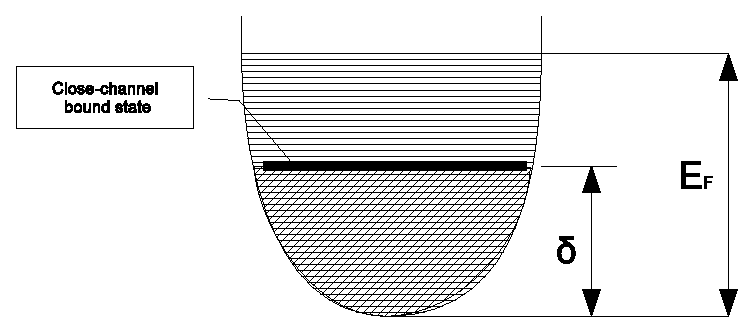
\includegraphics[width=.50\textwidth]{image/narrowFR.eps}
	\caption{Narrow Resonance\label{fig:narrowFR}}
\end{figure}
Fig. (\ref{fig:narrowFR}).  Here the zero-energy T-matrix is less  physically relevant than those with finite $T(E_{F}-\delta)$.  The more commonly used s-wave scattering length $a_{s}(E)$ likely changes sign within Fermi sea.  $T(E)$ dose not depends on $a_{s}(E)$, but also on effective range $r_{0}$.  

Here BCS/BEC extreme are subtle in the meaning.  If that refers to close-channel bound-state above or below Fermi sea.  Then the interaction is necessarily small as the condition for narrow resonance.  The more interesting part where it sits in the Fermi sea is always the middle case.  
